\chapter{Resultados}




A montagem do sistema de \textit{Hammerstein}, permitiu que fosse criada um modelo virtual do amplificador. Para verificar o funcionamento e performance do sistema criado, foi utilizado um único sinal de entrada para o amplificador real e o modelo virtual. O sinal de teste aplicado foi uma senoide de 1 kHz, mostrada na figura \ref{fig:tccfig}, na parte superior da imagem. Na parte inferior da figura \ref{fig:tccfig}, em azul está plotado a saída gravada do amplificador físico, em laranja, sobrepondo quase que por completo a cor azul, é a saída do modelo virtual do amplificador.

\begin{figure}
	\centering
	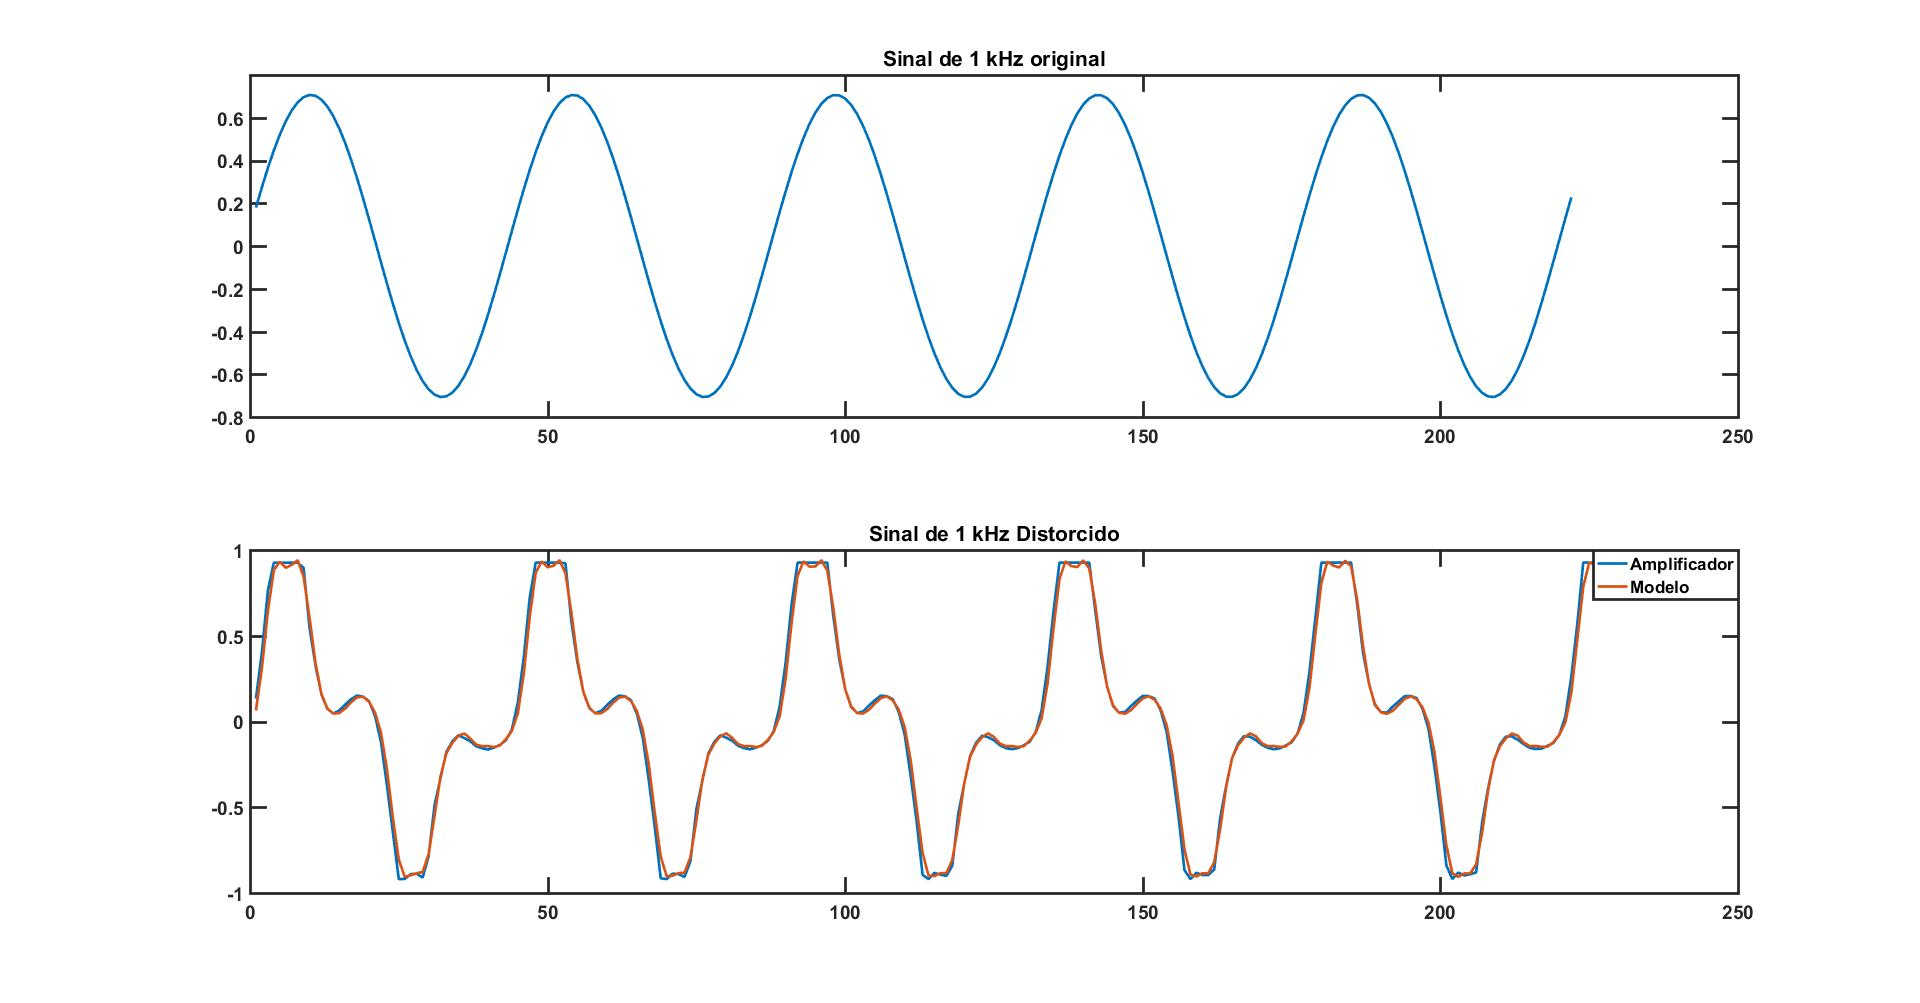
\includegraphics[width=1\linewidth]{figuras/TCC_fig}
	\caption{Superior: Sinal senoidal de 1 kHz utilizado para testar os modelos. Inferior: Em azul está o sinal distorcido pelo amplificador físico, em laranja a saída do modelo de \textit{Hammerstein}}
	\label{fig:tccfig}
\end{figure}

Para medir valores mais concretos entre as saídas gravadas do modelo real e físico, foi aplicado aos sinais gravados de cada modelo, a Transformada de Fourier para visualizar a resposta em frequência dos amplificadores. Na figura \ref{fig:tcc2fft}, na parte superior é mostrada a resposta frequencial do amplificador físico, já na parte inferior, a resposta frequencial do modelo. Através desse tipo de análise, é possível ter uma ideia das diferenças de intensidade entre os harmônicos gerados pelo modelo físico e pelo modelo de \textit{Hammerstein}. A tabela \ref{tab01}, mostra as medidas realizadas para cada harmônico entre os modelos, como se trata de um valor de intensidade de som, a unidade utilizada para os valores está de \textit{decibels}.
\begin{table}[h]
	\centering
	\caption{Propriedades obtidades após processamento}
	\label{tab01}
	
	\begin{tabular}{ccccc}
		\toprule
		\textbf{Harmônico} & \textbf{Amplificador (dB)} & \textbf{Modelo(dB)} & \textbf{Diferença (dB)} & \textbf{\% erro}  \\
		\midrule
		Fundamental & 48,20 & 48,36 & -0,16 & 0\% \\
		2º & 39,06 & 38,99 & 0,06 & 0\%  \\
		3º & 16,1 & 45,67 & 0,43 & 1\% 	\\
		4º & 37,09 & 37,65 & -0,56 & -2\% \\
		5º & 33,45 & 34,60 & -1,15 & -3\% \\ 
		6º & 33,73 & 31,84 & 1,89 & 6\%   \\ 
		7º & 36,68 & 36,42 & 0,26 & 1\%   \\ 
		8º & 35,49 & 34,22 & 1,27 & 4\%   \\ 
		9º & 35,90 & 34,84 & 1,06 & 3\%   \\ 
		10º & 32,44 & 32,06 & 0,37 & 1\%  \\ 
		11º & 32,07 & 30,67 & 1,39 & 4\%  \\
		\bottomrule
	\end{tabular}
	\label{Resultados obtidos}
	\caption{Resultados obtidos}
\end{table}

Os dados das tabelas mostram pequenas divergências entre os modelos, como no sexto harmônico, onde foi obtido o maior erro entre todos. Alguns harmônicos, como no caso do Fundamental e de outros, ultrapassa o valor do harmônico produzido pelo amplificador real. Por se tratar de uma digitalização, passando de um meio físico para um meio virtual, pela utilização de cabos e conectores e de uma interface de áudio, que realiza uma amostragem do sinal através de um conversor analógico digital, é de extrema dificuldade criar um modelo fiel, que consiga modificar o som de modo idêntico ao amplificador real, porém esse modelo pode alcançar resultados próximos o suficiente, possibilitando o uso de modelos desenvolvidos através dessa técnica.



\begin{figure}[!htb]
	\centering
	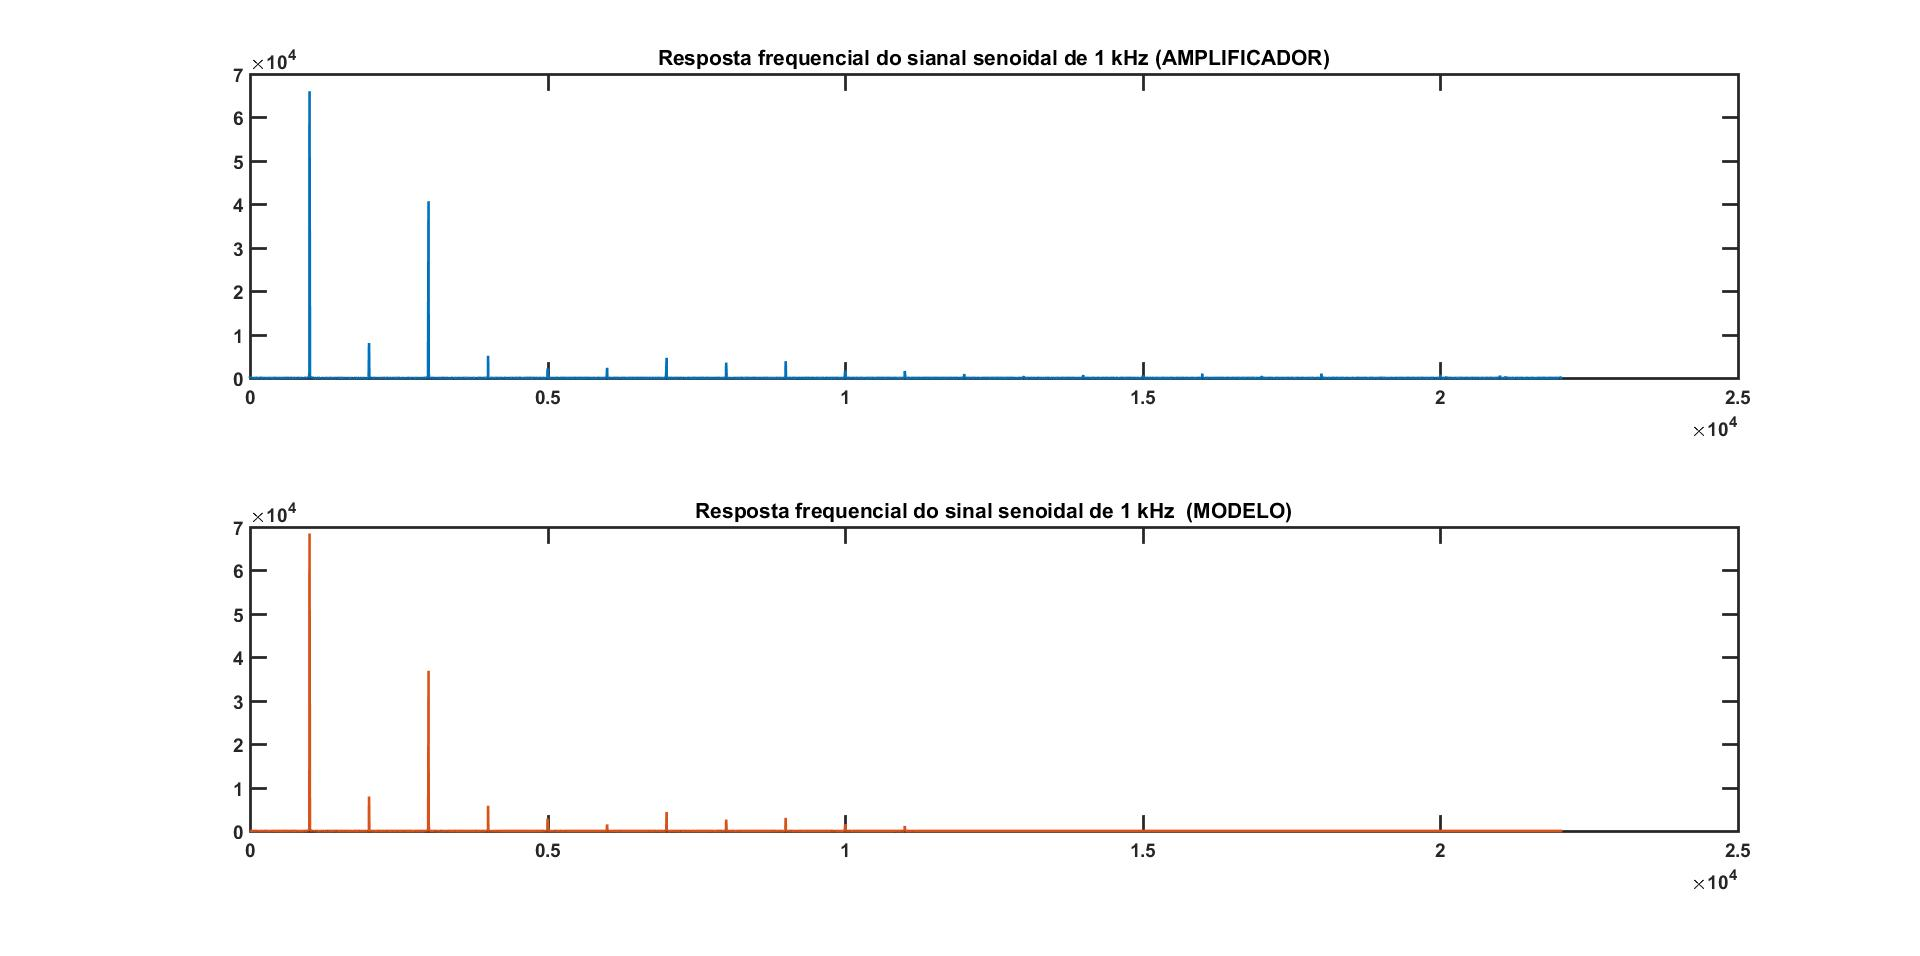
\includegraphics[width=1\linewidth]{figuras/Resp_freq}
	\caption{Resposta em frequência dos modelos}
	\label{fig:tcc2fft}
\end{figure}
Além de todos os equipamentos, cabos e conectores utilizados para a gravação dos sinais, existe uma relação máxima entre a ordem do modelo e a viabilidade de separação dos \kernels. O primeiro \textit{kernel}, observado bem no centro da figura \ref{fig:10sweepkernels} é separado por uma distância razoável do segundo \textit{kernel}, mas com o passar dos \kernels essa distância diminui, assim como suas intensidades, podendo ser considerado apenas ruído. A separação entre eles é dada pela equação \ref{kernel}, onde o $\Delta t_{m}$ é definido por:
\begin{equation}
\Delta t_{m} =  L \ln(m),
\label{eq:Delta_t_m}
\end{equation}

O parâmetro L na equação \ref{eq:Delta_t_m} é definido pelos parâmetros iniciais do sinal de excitação do sistema durante a caracterização e pode ser calculado através da equação \ref{Equação 5.10}
\begin{figure}
	\centering
	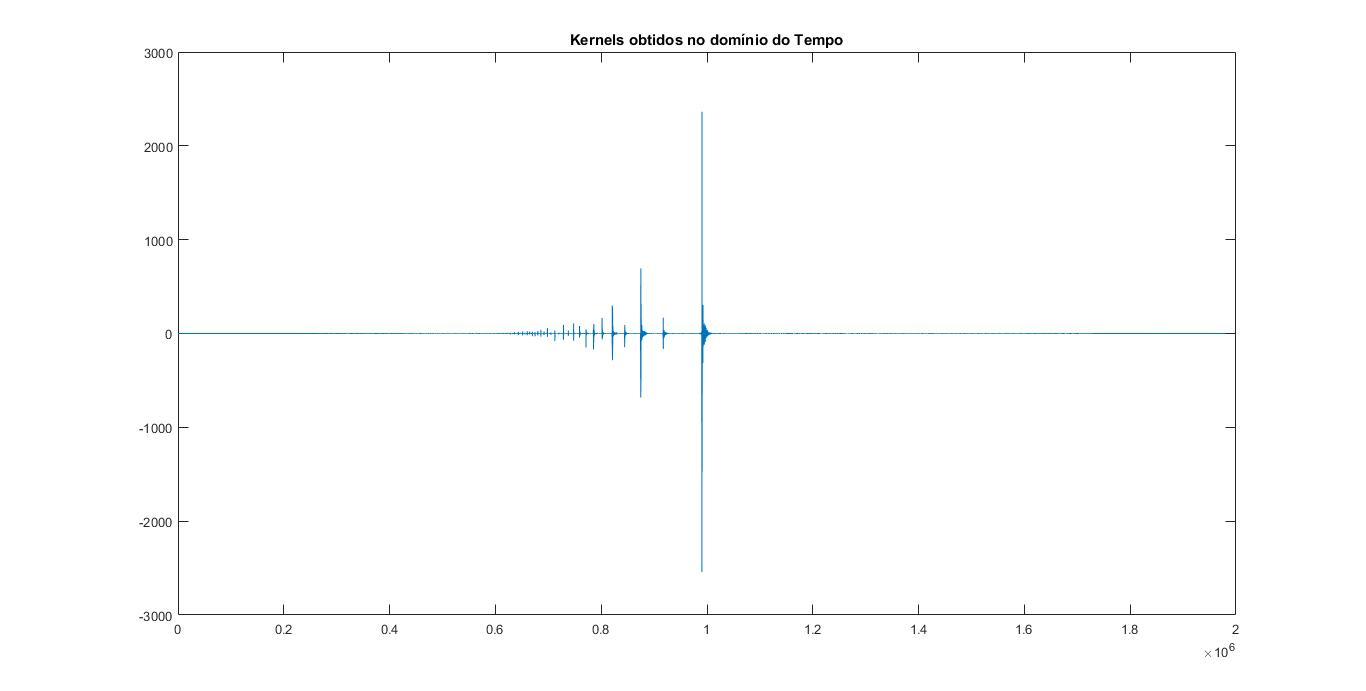
\includegraphics[width=0.7\linewidth]{figuras/10Sweep_Kernels}
	\caption{\kernels obtidos}
	\label{fig:10sweepkernels}
\end{figure}

Além da intensidade dos \kernels diminuir, eles tendem a estreitar os espaços, dificultando a separação de cada \textit{kernel} com a utilização de sistemas que utilizam ordens elevadas.
